\UseRawInputEncoding
\documentclass[12pt]{article}
\title{ECE 102 Homework 6}
\usepackage{subcaption}
\author{Lawrence Liu}
\usepackage{graphicx}
\usepackage{amsmath}
\usepackage[scr]{rsfso}

\newcommand{\Laplace}{\mathscr{L}}
\setlength{\parskip}{\baselineskip}%
\setlength{\parindent}{0pt}%
\usepackage{xcolor}
\usepackage{listings}
\definecolor{backcolour}{rgb}{0.95,0.95,0.92}
\usepackage{amssymb}
\lstdefinestyle{mystyle}{
    backgroundcolor=\color{backcolour}}
\lstset{style=mystyle}

\begin{document}
\maketitle
\section{Problem 1}
\subsection*{(a)}
We have
\begin{align*}
\int_0^t y(t-\tau)\tau^2e^{3-\tau} d\tau &=\int_{-\infty}^{\infty}\tau^2e^{3-\tau}y(t-\tau)u(t-\tau)d\tau\\ 
&=\left(t^2e^{3-t}u(t)\right)*y(t)\\
&\to \left(\frac{2e^3}{(s+1)^3}\right)Y(s)
\end{align*}
Thus we have
$$sY(s)+\left(\frac{2e^3}{(s+1)^3}\right)Y(s)=sX(s)-X(s)$$
And thus we have
$$H(s)=\frac{Y(s)}{X(s)}=\frac{s-1}{s+\frac{2e^3}{(s+1)^3}}$$
\subsection*{(b)}
The Fourier coefficients of $x(t)$ is
$$a_k=\begin{cases}
1.5 & k=0\\
\frac{1}{4} & |k|=2\\
0 & \text{everwhere else}
\end{cases}
$$

Therefore we have that the fourier series coefficients of $y(t)$, $b_k$ are
$$b_k=H(j)a_k=\begin{cases}
1.5\frac{j-1}{j+\frac{2e^3}{(j+1)^3}}& k=0\\
\frac{1}{4}\frac{j-1}{j+\frac{2e^3}{(j+1)^3}} & |k|=2\\
0 & \text{everwhere else}
\end{cases}$$
\subsection*{(c)}
From the fourier series properties,  given that
$$y(t)\to b_k$$
we have
\begin{align*}
y(t-3) &\to b_k e^{-6jk}\\
y(2t) &\to b_k\\
y(t-3)*y(2t) &\to b_k^2 e^{-6jk}\\
\end{align*}
\section*{Problem 2}
\subsection*{(a)}
\begin{align*}
X_1(j\omega)&=\int_{-\infty}^{+\infty} x_1(t)e^{-j\omega t}dt\\
&=\int_{0}^{1}t^2e^{-j\omega t}dt\\
&=\dfrac{\left(j{\omega}^2+2{\omega}-2j\right)\mathrm{e}^{-j{\omega}t}+2j}{{\omega}^3}
\end{align*}
\subsection*{(b)}
\begin{align*}
X_2(j\omega)&=\int_{-\infty}^{+\infty} x_2(t)e^{-j\omega t}dt\\
&=2\pi\delta(\omega)+\int_{-2}^{2}\cos(100t)e^{-j\omega t}dt\\
&=2\pi\delta(\omega)+\dfrac{\mathrm{e}^{-2j{\omega}}\cdot\left(\left(\cos\left(200\right)\,j{\omega}+100\sin\left(200\right)\right)\mathrm{e}^{4j{\omega}}-\cos\left(200\right)\,j{\omega}+100\sin\left(200\right)\right)}{10000-{\omega}^2}
\end{align*}
\subsection*{(c)}
\begin{align*}
\int_{-\infty}^t \cos(5(t-\sigma))\delta(\sigma-2)d\sigma &= \cos(5(t-2))\int_{-\infty}^t\delta(\sigma-2)d\sigma
\end{align*}
We have that
\begin{align*}
\cos(t)&\to \pi (\delta (\omega-1)+\delta(\omega+1))\\
\cos(t-2)&\to \pi e^{-2j\omega} (\delta (\omega-1)+\delta(\omega+1))\\
\cos(5(t-2))&\to \frac{\pi}{5} e^{-2j\frac{\omega}{5}} (\delta (\frac{\omega}{5}-1)+\delta(\frac{\omega}{5}+1))\\
&=\pi e^{-2j}\delta (\omega-5)+\pi e^{2j}\delta (\omega+5)
\end{align*}

\begin{align*}
\cos(5(t-2))\int_{-\infty}^t\delta(\sigma-2)d\sigma&\to \left(\pi e^{-2j}\delta (\omega-5)+\pi e^{2j}\delta (\omega+5)\right)*\left(\frac{e^{-2j\omega}}{j\omega}+\pi \delta(\omega)\right)\\
&=\pi e^{-2j}\left(\frac{e^{-2j(\omega-5)}}{j(\omega-5)}+\pi\right)\delta (\omega-5)+\pi e^{2j}\left(\frac{e^{-2j(\omega+5)}}{j(\omega+5)}+\pi\right)\delta (\omega+5)
\end{align*}
\section*{Problem 3}
\subsection*{(a)}
\begin{align*}
X(0)&=\int_{-\infty}^{\infty}x(t)dt\\
&=6
\end{align*}
Likewise, since $$\int_{-\infty}^{\infty} \frac{1}{j\omega}+\pi\delta(\omega)d\omega=\pi$$
And 
$$x(t)=u(t+1)+u(t)-u(t-2)-u(t-3)$$
Thus we have
$$\int_{-\infty}^{\infty}X(j\omega)d\omega=3\pi$$
\subsection*{(b)}
We know that
$$\int_{-\infty}^{\infty}\left|x(t)\right|^2dt=10$$
Thus from Parseval's Reltaion we have
$$\int_{-\infty}^{\infty}\left|X(j\omega)\right|^2 d\omega=20\pi$$
\subsection*{(c)}
We have
$$\frac{2\sin(\omega)}{\omega}\to\begin{cases}
1 & |t|<1\\
0 & |t|>1
\end{cases}$$
$$e^{j2\omega}\frac{2\sin(\omega)}{\omega}\to y(t)=\begin{cases}
1 & -3<t<-1\\
0 & \text{elsewhere}
\end{cases}$$
Thus we have
$$y(-t)=\begin{cases}
1 & 1<t<3\\
0 & \text{elsewhere}\end{cases}$$
Therefore we have
$$\int_{-\infty}^{\infty}X(\omega)Y(\omega)d\omega=2\pi\int_{-\infty}^{\infty} x(t)y(-t)dt=6\pi$$
\subsection*{(d)}
The inverse Fourier transform of $Re\{X(j\omega)\}$ is the even part of $x(t)$ or
$$u(t+3)+u(t+2)+u(t+1)-u(t-1)-u(t-2)-u(t-3)$$
The plot of which looks like
\begin{center}
\begin{figure}[h]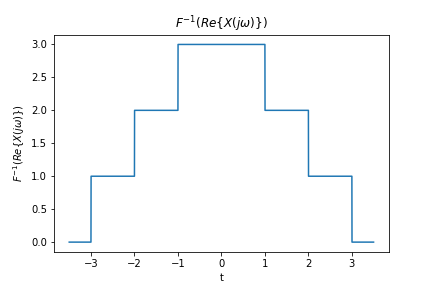
\includegraphics[width=8cm]{fig1}
\end{figure}
\end{center}
\section*{Problem 4}
From condition 1 and 2 we know that 
$x(t)$ must be of the form 
$$x(t)=-ce^{-2t}u(t)+ce^{-t}u(t)$$
From condition 3 we have
$$\int_{-\infty}^{+\infty}|X(j\omega)|^2d\omega=2\pi$$
Therefore, from parseval's we have
\begin{align*}
\int_{-\infty}^{+\infty}|x(t)|^2dt&=1\\
c^2\int_{0}^{+\infty}e^{-4t}dt+2c^2\int_{0}^{+\infty}e^{-3t}dt+c^2\int_{0}^{+\infty}e^{-2t}dt&=1\\
\frac{c^2}{4}-\frac{2c^2}{3}+\frac{c^2}{2}&=1\\
\end{align*}
Thus we have $c=2\sqrt{3}$, $x(t)=2\sqrt{3}(e^{-t}-e^{-2t})u(t)$ and thus $A=-2\sqrt{3}$
\section*{Problem 5}
\subsection*{(a)}
$$X(s)=\frac{2\pi}{(s+1)^2+4\pi^2}+e^{-2s}$$
$$X(j\omega)=\frac{2\pi}{(j\omega+1)^2+4\pi^2}+e^{-2j\omega}$$
\subsection*{(b)}
We have that
$$|X(j\omega)|^2=\sqrt{X(j\omega)X^*(j\omega)}$$
Since $x(t)$ is real we have
$$X*(j\omega)=X(-j\omega)$$
Therefore we have
\begin{align*}
|X(j\omega)|^2&=\left(\frac{2\pi}{(j\omega+1)^2+4\pi^2}+e^{-2j\omega}\right)\left(\frac{2\pi}{(-j\omega+1)^2+4\pi^2}+e^{2j\omega}\right)\\
|X(j\omega)|&=\sqrt{\left(\frac{2\pi}{(j\omega+1)^2+4\pi^2}+e^{-2j\omega}\right)\left(\frac{2\pi}{(-j\omega+1)^2+4\pi^2}+e^{2j\omega}\right)}
\end{align*}
if $X(j\omega)+X(-j\omega)\geq0$ we have
\begin{align*}
\measuredangle X(j\omega)&=\arctan\left( \frac{X(j\omega)-X(-j\omega)}{i(X(j\omega)+X(-j\omega)}\right)\\
&=\arctan\left(\frac{-2\sin(2\omega)(\omega^{4} - 8 \pi^{2} \omega^{2} + 2 \omega^{2} + 1 + 8 \pi^{2} + 16 \pi^{4})-8 \pi \omega}{2\cos(2\omega)(\omega^{4} - 8 \pi^{2} \omega^{2} + 2 \omega^{2} + 1 + 8 \pi^{2} + 16 \pi^{4})+4 \pi \left(- \omega^{2} + 1 + 4 \pi^{2}\right)}\right)
\end{align*}
And if $X(j\omega)+X(-j\omega)<0$ we have
$$
\measuredangle X(j\omega)=\arctan\left(\frac{-2\sin(2\omega)(\omega^{4} - 8 \pi^{2} \omega^{2} + 2 \omega^{2} + 1 + 8 \pi^{2} + 16 \pi^{4})-8 \pi \omega}{2\cos(2\omega)(\omega^{4} - 8 \pi^{2} \omega^{2} + 2 \omega^{2} + 1 + 8 \pi^{2} + 16 \pi^{4})+4 \pi \left(- \omega^{2} + 1 + 4 \pi^{2}\right)}\right)+\pi$$

\subsection*{(c)}
using this code, we get
\lstinputlisting[language=Matlab]{Problem5c.m}
\begin{center}
\begin{figure}[h]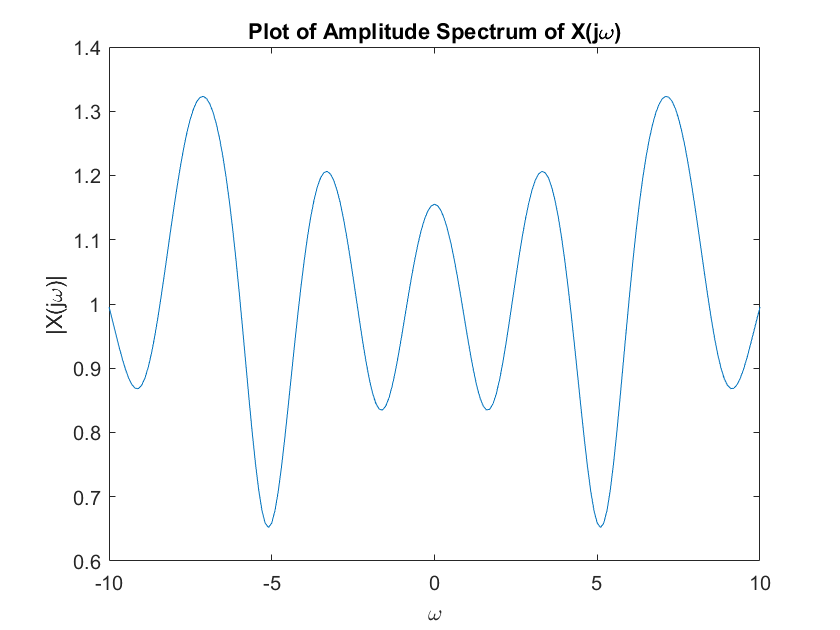
\includegraphics[width=8cm]{fig2}
\end{figure}
\end{center}
\begin{center}
\begin{figure}[h]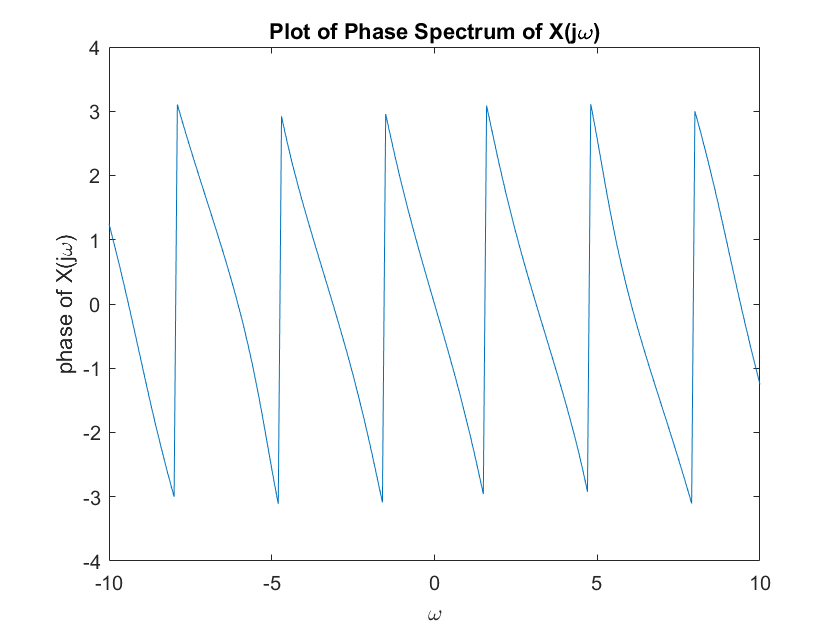
\includegraphics[width=8cm]{fig3}
\end{figure}
\end{center}
\end{document}